\section{Direct forecasting ablation of geometric soft-state observables}
\label{sec:soft-state-ablation-supp}

\paragraph{Production and verification status.}
Source publication, the fixed \SATasks-task cohort, target release, and
the frozen analysis are complete. The independent computational audit
passed for every task. Its achieved coverage and numerical tolerances
are reported below, alongside all four primary outcomes and the
descriptive secondary results.

This study isolates three layers of the forecasting representation:
membership in reference regions, position within those regions, and
reconstruction departures. It compares four direct readouts of the same
future observations. Its question differs from whether a correction
improves a retained baseline or a forecasting selection policy. The
readouts here have access only to their declared representation.
The source, configuration, and analysis contract are retained under
\path{extensions/soft_state_ablation_20261102/}.
Earlier studies informed the design; their terminal losses are not pooled
with this cohort. Fresh simulation repetitions provide new evaluation
units under familiar laws, rather than new application domains or
independent hypothesis discovery.

\subsection{Observation laws and allocation}

The factorial design crosses \SARepetitions\ independent repetitions,
four laws, and two added-noise levels, giving \SATasks\ task suites.
The nonlinear autoregression, Van der Pol, and Duffing observation laws
are exactly those specified in Appendix~\ref{c:app:methods}, including
initial-state distributions, integration, burn-in, and sensor noise.
Only those generator specifications are inherited; the allocation below
replaces the earlier study's sample sizes. The linear negative control is
\[
 u_t=0.65u_{t-1}-0.15u_{t-2}+\epsilon_t,
 \qquad \epsilon_t\stackrel{\mathrm{iid}}\sim N(0,0.1^2),
\]
initialized at zero for two stored values and retaining seventy-two
values after discarding the first $256$.

For each law and repetition, independent episode sets A/B/C/D contain
$64/32/32/128$ episodes. Add $\eta s_A e_t$ to each stored observation,
where $\eta\in\{0,0.1\}$, $e_t$ is standard Gaussian, and $s_A$ is the
population standard deviation of all original A episode values.
The same augmentation affects histories and targets. The oscillator
observations already contain sensor noise when $\eta=0$.
Zero-based origins are $t=11,15,\ldots,59$; each input is
$(y_{t-11},\ldots,y_t)^\top$ and each target is
$(y_{t+1},y_{t+4},y_{t+12})^\top$.
Uniform sampling without replacement retains at most $512/256/256$
rows on A/B/C. D retains all thirteen origins from each episode,
giving $1{,}664$ rows. Origins within an episode overlap and are dependent.

Master seed $2026110203$ and the frozen integer-component NumPy
\texttt{SeedSequence} rule define $1{,}696$ intended-distinct streams.
Generation, unit noise, row retention, and fitting are paired across
noise levels and competitors. Split-specific streams separate A/B/C/D.
The complete roster was checked internally and against the recorded
historical exclusions before generation. No old cohort was relabeled as
fresh evidence. The repetition count and candidate menu remained fixed
through terminal evaluation.

\subsection{Shared native geometry and block-preserving representations}

Each candidate bank uses A-fitted standardization, partitions requesting
$2,4,8$ groups, at most twenty-four references per local model, and the
$512$-row bank limit. The input-scaling convention is fixed; there is no
scaler search. At requested cap $c$, ambient dimension $d=12$, and local
reference count $n_j$, native initialization is
$r_j^{\mathrm{init}}=\min\{c,d,n_j-1\}$.
Positive-variance and projected-coordinate-range checks can reduce the
stored rank. The range rule stops at requested rank one; a model with
no admissible positive-variance direction retains the explicit rank-zero
wrapper. Full ambient rank is permitted, without an additional $d-1$
restriction. The grid is $c\in\{1,2,4,8,12\}$; cap twenty is an alias
of twelve at this history width and is checked on artificial data rather
than counted as another search opportunity.

For standardized history $z$, local center $\mu_j$, basis $P_j$, and
squared-radius scale $s_j$, the gates within partition $\mathcal J_b$ are
\[
 g_j(z)=\frac{\exp\{-\|z-\mu_j\|_2^2/(2s_j)\}}
 {\sum_{\ell\in\mathcal J_b}
       \exp\{-\|z-\mu_\ell\|_2^2/(2s_\ell)\}}.
\]
The raw common matrix places all gates first, followed by the blocks
$g_j(z)P_j^\top(z-\mu_j)$ in local-model order. Denote these two
parts by $g(z)$ and $\ell(z)$. The untransformed gates sum to one
within each partition; their concatenation lies in a product of
simplexes. This property does not apply to the signed position or
departure coordinates, or generally to the transformed readout vector.

At positive rank, with projected-reference sample covariance $S_j$,
the Gaussian kernel is
\[
 \kappa_j(z,z')=\exp\!\left\{
 -\frac{[P_j^\top(z-z')]^\top S_j^{-1}P_j^\top(z-z')}{2r_j}
 \right\}.
\]
With transformed references as rows of $Q_j$, query kernel $k_j$,
Gram matrix $K_j$, and reference-fitted regularizer $\lambda_j>0$,
the matched reconstructions are
\[
 A_{K,j}(z)=\frac{Q_j^\top C_jk_j(z)}{\mathbf1^\top C_jk_j(z)},
 \quad A_{R,j}(z)=\frac{Q_j^\top k_j(z)}{\mathbf1^\top k_j(z)},
 \quad C_j=(K_j+\lambda_jI)^{-1}.
\]
The kernel and regularizer retain the native implementation. Both
departures subtract
$A_{A,j}(z)=\mu_j+P_jP_j^\top(z-\mu_j)$ and stack
$g_j(z)\{A_{m,j}(z)-A_{A,j}(z)\}$ over models, for $m=K,R$.
They retain all ambient coordinates. K and R share references, projected
kernels, gates, and departure width within each bank.
The inherited relative-denominator threshold $10^{-10}$ and finite-value
guards remain active. Affine fallback makes the affected raw departure
zero; it need not remain zero after feature centering.

Each of the four raw blocks $g,\ell,d_K,d_R$ receives its own A-fitted
column centering and scaling, with scale floor $10^{-6}$, followed by
\begin{equation}
 T_p(v)=\frac{v}{\sqrt{1+\|v\|_2^2/p}},\qquad p>0.
 \label{eq:supp-sa-block-map}
\end{equation}
An empty block stays empty. A tilde denotes this complete block
transformation. Table~\ref{supp:sa-architecture} gives the readout inputs.
There is no subsequent normalization of a concatenated descriptor.
The transformed gate block is therefore identical in all arms, and
the position block is identical in P/K/R. Exact prefix hashes check
these identities. Separately transforming the blocks defines a new
procedure: older results that bound the complete common vector are not
results for this ablation.

\begin{table}[t]
\centering\small
\caption{Four direct forecasting representations at a fixed shared bank.
The table specifies available coordinates, not a claim of equal capacity
or of predictive sufficiency.}
\label{supp:sa-architecture}
\begin{tabular}{@{}p{0.08\linewidth}p{0.40\linewidth}p{0.44\linewidth}@{}}
\toprule
Arm & Readout input & Added predictive content being tested \\
\midrule
G & $\widetilde g$ & Relative membership in reference regions. \\
P & $(\widetilde g,\widetilde\ell)$ & Position within the same regions. \\
K & $(\widetilde g,\widetilde\ell,\widetilde d_K)$ & Inverse-Gram reconstruction departures. \\
R & $(\widetilde g,\widetilde\ell,\widetilde d_R)$ & Matched positive-kernel departures. \\
\bottomrule
\end{tabular}
\end{table}

\subsection{Readout fitting and cap selection}

For each cap, arm, and horizon, A fits the affine ridge objective
\[
 \min_{a,w}\;\frac1{n_A}\sum_{i\in A}
       \{y_{ih}-a-f(x_i)^\top w\}^2+\alpha\|w\|_2^2,
 \qquad \alpha\in\{10^{-4},10^{-3},10^{-2},10^{-1},1\},
\]
where $f$ is the declared representation and the intercept is unpenalized.
The target is the observed future value, with no retained raw-history
forecast, residual target, or correction multiplier. B independently
selects each horizon's penalty. Each arm supplies twenty-five B
candidate scores per horizon across the five caps.

The primary comparison uses one shared cap: P minimizes its B MSE,
normalized by the corresponding retained-A target population variance
floored at $10^{-12}$, and averaged equally across horizons. All four
arms use that bank with their own selected penalties. Exact ties retain
the first candidate in ascending cap or penalty order. The secondary
view lets each arm select its own cap from the same candidate fits.
It addresses complete-procedure performance rather than the primary
shared-geometry question. Equal K/R widths and search counts do not
equate function classes, conditioning, computation, or statistical
capacity. Larger representations also need not constitute compression.

The inherited centered-SVD solver is retained. Only its documented
linear-algebra exception invokes the checked SciPy \texttt{gesvd}
recovery, preserving the objective and recording the event. Unhandled
failures stop the study; tasks are not discarded or silently replaced.
C is diagnostic only: every choice and fitted state is saved before
its histories and targets are accessed for diagnostic predictions and
losses. C performs no fitting, calibration, or selection.

\subsection{Losses and the complete primary family}

For task $\tau$, arm $m$, and horizon $h$, let
\[
 v_{\tau h}=\max\{\operatorname{Var}_{A,\tau}(Y_h),10^{-12}\},
 \qquad
 L_{\tau m}=\frac13\sum_{h\in\{1,4,12\}}
 \frac{n_D^{-1}\sum_{i\in D}(y_{ih}-\widehat y_{m,ih})^2}{v_{\tau h}}.
\]
Within each repetition, average the six nonlinear law/noise cells
equally, or the two linear cells for the separate negative-control panel.
Only the $n=\SARepetitions$ complete repetition aggregates are treated
as independent units. Horizons, local models, origins, and paired noise
levels do not enlarge that sample size.

The four primary shared-bank differences are
\[
 \begin{array}{ll}
 L_{r,P}^{\mathrm{NL}}-0.97L_{r,G}^{\mathrm{NL}}, &
 L_{r,K}^{\mathrm{NL}}-0.97L_{r,P}^{\mathrm{NL}},\\
 L_{r,K}^{\mathrm{NL}}-0.97L_{r,R}^{\mathrm{NL}}, &
 L_{r,K}^{\mathrm{lin}}-1.05L_{r,P}^{\mathrm{lin}}.
 \end{array}
\]
For each difference sequence $d_r$, the decision is
\begin{equation}
 U=\bar d+t_{n-1,1-0.05/4}\frac{s_d}{\sqrt n}<0,
 \label{eq:supp-sa-primary}
\end{equation}
with sample standard deviation $s_d$ and $n-1=31$ degrees of freedom;
$t_{\nu,p}$ denotes the $p$ quantile with $\nu$ degrees of freedom.
These one-sided Bonferroni bounds form a single four-claim family under
the paired-mean Student approximation; they are not distribution-free
certificates. The 3\% improvement and 5\% noninferiority margins are
research conventions, not deployment-derived tolerances.
Percentage gains use ratios of mean losses. Secondary independent-cap,
law/noise, horizon, and paired-difference summaries remain descriptive;
any ordinary 95\% intervals are unadjusted. Every primary contrast is
reported, and failure to establish a margin does not establish equality.

\subsection{Staging, retained evidence, and audit scope}

The recorded production order was source/configuration/analysis freeze, verified
source publication and its commit-bound receipt, complete A/B/C
preparation, fitting and a global fit seal, D generation into separate
query and target archives, query-only prediction and a global prediction
seal, target release, analysis, and independent audit.
Three fresh-process workers used one numerical thread each.
Production preparation required the publication receipt to match the
source freeze; subsequent manifests bound its hash.
These checks document procedural order and detect
changes, without providing cryptographic target isolation.

Portable JSON/NPZ states retain the geometry, block transforms, and
coefficients. The records include every B penalty path, both selected
views, diagnostic C predictions, eight D forecast matrices per task,
local-rank audits, numerical guards, and resource measurements.
Whole-task costs include rejected candidates and shared computations;
they are not isolated deployed-model costs. Recorded peak resident
memory is per worker, rather than aggregate concurrent memory.

Artificial-data preflight exercised block identity, native cap aliases,
rank-zero behavior, ridge solutions, portable-state replay, and the stage
gates. The independent audit reconstructed histories from retained
episodes and reserved noise/row streams, refitted all B penalty paths
using Cholesky normal equations, replayed selected C/D forecasts,
checked native rank/kernel identities, and recomputed all primary
statistics. It did not independently reimplement partition fitting or
physical-law integration. The completed receipt records achieved
coverage and numerical tolerances.
Computational verification also does not constitute external scientific
replication. The study evaluates finite direct-readout utility, without
testing autonomous state propagation, Markov sufficiency, exact Koopman
closure, or a universal KAHM advantage.

\FloatBarrier
\subsection{Complete primary results}

All \SATasks\ task suites contributed their eight forecasts to the
released analysis; the inferential sample remains \SARepetitions\
complete repetitions. Tables~\ref{supp:sa-aggregate} and
\ref{supp:sa-primary} give both cap-selection views and the complete
prespecified primary family. In the shared-cap nonlinear panel, adding
local position to membership reduced mean SMSE by \SAGainPG\%, and
adding KAHM departures to position reduced it by \SAGainKP\%.
Both 3\% superiority criteria were established. P improved on G and
K improved on P in all thirty-two nonlinear repetition aggregates.
These are comparisons of fitted direct readouts; their larger feature
sets also give them more coordinates and different regularization
behavior.

The matched K/R result limits the KAHM-specific conclusion. Their
nonlinear mean SMSEs were $0.0272660$ and $0.0272740$, respectively,
giving only \SAGainKR\% point improvement for K. The upper bound for
$L_K-0.97L_R$ was positive, and the 3\% superiority criterion was not
established. K had lower loss in eighteen of thirty-two repetitions.
This finding does not establish equivalence or show that the two maps
are interchangeable. It shows that this cohort does not establish the
prespecified additional advantage of inverse-Gram reconstruction over
its matched positive-kernel control.

The linear control also prevents an unqualified improvement claim:
K's mean SMSE was $0.921045$, compared with $0.910921$ for P, a
$1.11\%$ increase. The 5\% noninferiority criterion was established,
although K improved on P in only two of thirty-two repetitions.
Thus three of the four primary criteria were established. The linear
result concerns a tolerated loss increase under the stated research
margin; it is not linear-control superiority.

\begin{table}[t]
\centering\small
\caption{Complete D aggregates for the representation-only ablation.
SMSE is averaged over horizons, then equally over the six nonlinear or
two linear law/noise cells within each repetition. SD is across the
\SARepetitions\ complete repetitions, not a confidence interval.
The independent-cap view is secondary.}
\label{supp:sa-aggregate}
% Generated by build_soft_state_assets.py; do not edit.
% D SMSE; SD across 32 complete repetitions, not a confidence interval. Independent caps are secondary.
\begin{tabular}{@{}llrrrr@{}}
\toprule
Cap rule & Arm & Nonlinear mean & SD & Linear mean & SD \\
\midrule
Shared & G & 0.0988703 & 0.00788637 & 0.939042 & 0.0484704 \\
Shared & P & 0.0304507 & 0.00150099 & 0.910921 & 0.0513907 \\
Shared & K & 0.027266 & 0.00123317 & 0.921045 & 0.0526607 \\
Shared & R & 0.027274 & 0.00127755 & 0.915866 & 0.0512334 \\
\addlinespace
Independent & G & 0.0988703 & 0.00788637 & 0.939042 & 0.0484704 \\
Independent & P & 0.0304507 & 0.00150099 & 0.910921 & 0.0513907 \\
Independent & K & 0.0267546 & 0.00120524 & 0.914936 & 0.0511589 \\
Independent & R & 0.0267507 & 0.00129299 & 0.91589 & 0.0521994 \\
\bottomrule
\end{tabular}

\end{table}

\begin{table}[t]
\centering\small
\caption{All four primary shared-cap comparisons. Gain is
$100(1-\overline L_{\mathrm{candidate}}/
\overline L_{\mathrm{reference}})$.
The margin-adjusted difference and its simultaneous one-sided upper
bound are in absolute SMSE units, not percentages. The factors are
$0.97$ for nonlinear superiority (sup.) and $1.05$ for linear
noninferiority (NI); a criterion is met only when its upper bound is
strictly negative. The four bounds use Equation~\eqref{eq:supp-sa-primary}.}
\label{supp:sa-primary}
% Generated by build_soft_state_assets.py; do not edit.
% Shared caps; d=L_candidate-factor*L_reference. Four Bonferroni one-sided paired-t upper bounds; met iff upper<0.
\begin{tabular}{@{}lllrrrc@{}}
\toprule
Population & Contrast & Criterion & Gain (\%) & $\bar d$ & Upper bound & Met \\
\midrule
Nonlinear & P vs G & 3\% sup. & 69.20 & \ensuremath{-0.06545} & \ensuremath{-0.06253} & Yes \\
Nonlinear & K vs P & 3\% sup. & 10.46 & \ensuremath{-0.002271} & \ensuremath{-0.001987} & Yes \\
Nonlinear & K vs R & 3\% sup. & 0.03 & 0.0008103 & 0.000981 & No \\
Linear & K vs P & 5\% NI & \ensuremath{-1.11} & \ensuremath{-0.03542} & \ensuremath{-0.03134} & Yes \\
\bottomrule
\end{tabular}

\end{table}

\FloatBarrier
\subsection{Descriptive cap-selection, condition, and horizon results}

Allowing each arm to select its own cap reduced nonlinear K and R
SMSE to $0.0267546$ and $0.0267507$, respectively. Their improvements
over P were $12.14\%$ and $12.15\%$. The corresponding K/R gain was
$-0.014\%$, slightly favoring R at the point-estimate level. Independent
selection reduced K's linear mean to $0.914936$, still above P.
The complete twenty-four descriptive comparisons, including changes
between cap-selection views, appear in Table~\ref{supp:sa-secondary}.
Their ordinary paired intervals are unadjusted and do not replace the
four primary decisions. In particular, neither a near-zero K/R point
difference nor an interval containing zero is an equivalence test.

The aggregate nonlinear benefit masks substantial variation
(Table~\ref{supp:sa-conditions} and Figure~\ref{supp:sa-condition-gains}).
Under shared caps, K worsened P on the nonlinear autoregression at
both added-noise levels, from $0.021445$ to $0.022615$ and from
$0.032966$ to $0.035102$. Both reconstruction arms improved P on
the Van der Pol and Duffing cells, while K outperformed R in only
three of the six nonlinear cells. For example, the no-added-noise
Van der Pol losses were $0.015168$ for P, $0.003281$ for K, and
$0.004678$ for R. On noisy Duffing, R had slightly lower loss than K.
These comparisons are descriptive findings under inherited laws;
they are not separately adjusted condition-specific discoveries.

Horizon-specific results also distinguish the tested finite-horizon
readouts from a propagation claim (Table~\ref{supp:sa-horizons}).
In the nonlinear shared-cap panel, K had slightly larger loss than P
at $h=1$ ($0.012639$ versus $0.012255$), nearly the same loss at
$h=4$ ($0.019227$ versus $0.019254$), and smaller loss at $h=12$
($0.049932$ versus $0.059843$). K was worse than R at the first
two horizons and better at the third. Each horizon has its own
fitted readout and selected penalty. No forecast in this comparison
is obtained by iterating an estimated state-transition operator.

\begin{table}[htbp]
\centering\small
\caption{All planned descriptive paired comparisons. The difference is
candidate minus reference without a practical-margin factor.
The ordinary 95\% intervals use \SARepetitions\ paired repetition
aggregates and are unadjusted. ``Ind.\ vs shared'' compares the two
cap-selection procedures for the same arm. These intervals do not
establish additional primary claims or equivalence.}
\label{supp:sa-secondary}
% Generated by build_soft_state_assets.py; do not edit.
% Unadjusted descriptive paired intervals; Delta=candidate-reference, with no practical margin. Cross-view rows compare independent minus shared for the same arm.
\begin{tabular}{@{}lllrrrr@{}}
\toprule
Population & Cap rule & Arm contrast & Gain (\%) & $\bar\Delta$ & 95\% lower & 95\% upper \\
\midrule
Nonlinear & Shared & P vs G & 69.20 & \ensuremath{-0.06842} & \ensuremath{-0.07103} & \ensuremath{-0.06581} \\
Nonlinear & Shared & K vs P & 10.46 & \ensuremath{-0.003185} & \ensuremath{-0.00344} & \ensuremath{-0.00293} \\
Nonlinear & Shared & K vs R & 0.03 & \ensuremath{-7.968\times 10^{-6}} & \ensuremath{-0.0001589} & 0.000143 \\
Nonlinear & Shared & R vs P & 10.43 & \ensuremath{-0.003177} & \ensuremath{-0.003391} & \ensuremath{-0.002962} \\
Nonlinear & Independent & P vs G & 69.20 & \ensuremath{-0.06842} & \ensuremath{-0.07103} & \ensuremath{-0.06581} \\
Nonlinear & Independent & K vs P & 12.14 & \ensuremath{-0.003696} & \ensuremath{-0.003961} & \ensuremath{-0.003431} \\
Nonlinear & Independent & K vs R & \ensuremath{-0.01} & \ensuremath{3.864\times 10^{-6}} & \ensuremath{-0.0001309} & 0.0001386 \\
Nonlinear & Independent & R vs P & 12.15 & \ensuremath{-0.0037} & \ensuremath{-0.003929} & \ensuremath{-0.003471} \\
Nonlinear & Ind. vs shared & G & 0.00 & 0 & 0 & 0 \\
Nonlinear & Ind. vs shared & P & 0.00 & 0 & 0 & 0 \\
Nonlinear & Ind. vs shared & K & 1.88 & \ensuremath{-0.0005114} & \ensuremath{-0.0007194} & \ensuremath{-0.0003034} \\
Nonlinear & Ind. vs shared & R & 1.92 & \ensuremath{-0.0005233} & \ensuremath{-0.0007183} & \ensuremath{-0.0003283} \\
\addlinespace
Linear & Shared & P vs G & 2.99 & \ensuremath{-0.02812} & \ensuremath{-0.03159} & \ensuremath{-0.02465} \\
Linear & Shared & K vs P & \ensuremath{-1.11} & 0.01012 & 0.006675 & 0.01357 \\
Linear & Shared & K vs R & \ensuremath{-0.57} & 0.005179 & 0.002502 & 0.007856 \\
Linear & Shared & R vs P & \ensuremath{-0.54} & 0.004945 & 0.003546 & 0.006343 \\
Linear & Independent & P vs G & 2.99 & \ensuremath{-0.02812} & \ensuremath{-0.03159} & \ensuremath{-0.02465} \\
Linear & Independent & K vs P & \ensuremath{-0.44} & 0.004015 & 0.001816 & 0.006214 \\
Linear & Independent & K vs R & 0.10 & \ensuremath{-0.0009539} & \ensuremath{-0.002991} & 0.001083 \\
Linear & Independent & R vs P & \ensuremath{-0.55} & 0.004969 & 0.003123 & 0.006815 \\
Linear & Ind. vs shared & G & 0.00 & 0 & 0 & 0 \\
Linear & Ind. vs shared & P & 0.00 & 0 & 0 & 0 \\
Linear & Ind. vs shared & K & 0.66 & \ensuremath{-0.006109} & \ensuremath{-0.008889} & \ensuremath{-0.003328} \\
Linear & Ind. vs shared & R & \ensuremath{-2.65\times 10^{-3}} & \ensuremath{2.431\times 10^{-5}} & \ensuremath{-0.00188} & 0.001929 \\
\bottomrule
\end{tabular}

\end{table}

\begin{table}[htbp]
\centering\small
\caption{Complete descriptive law/noise results for both cap-selection
views. Each cell is mean D SMSE over \SARepetitions\ repetitions and
three horizons. The noise parameter is the added-noise multiplier;
the underlying oscillator observations already contain sensor noise
when $\eta=0$. All eight conditions are retained.}
\label{supp:sa-conditions}
% Generated by build_soft_state_assets.py; do not edit.
% Descriptive D SMSE by law/noise; each mean uses all 32 repetitions and averages the three horizons.
\begin{tabular}{@{}llrrrrr@{}}
\toprule
Cap rule & Law & $\eta$ & G & P & K & R \\
\midrule
Shared & Nonlinear AR & 0 & 0.0244281 & 0.0214449 & 0.0226148 & 0.0217499 \\
Shared & Nonlinear AR & 0.1 & 0.0337124 & 0.0329659 & 0.0351019 & 0.0336442 \\
Shared & Van der Pol & 0 & 0.148037 & 0.0151678 & 0.00328116 & 0.00467759 \\
Shared & Van der Pol & 0.1 & 0.149308 & 0.0511417 & 0.0471983 & 0.0477871 \\
Shared & Duffing & 0 & 0.118935 & 0.0158738 & 0.0133303 & 0.0138744 \\
Shared & Duffing & 0.1 & 0.118801 & 0.0461102 & 0.0420697 & 0.0419106 \\
Shared & Linear AR & 0 & 0.937648 & 0.909514 & 0.918951 & 0.914566 \\
Shared & Linear AR & 0.1 & 0.940436 & 0.912328 & 0.923139 & 0.917166 \\
\addlinespace
Independent & Nonlinear AR & 0 & 0.0244281 & 0.0214449 & 0.0225847 & 0.0217757 \\
Independent & Nonlinear AR & 0.1 & 0.0337124 & 0.0329659 & 0.0348346 & 0.0335888 \\
Independent & Van der Pol & 0 & 0.148037 & 0.0151678 & 0.00252973 & 0.00347309 \\
Independent & Van der Pol & 0.1 & 0.149308 & 0.0511417 & 0.046256 & 0.0466229 \\
Independent & Duffing & 0 & 0.118935 & 0.0158738 & 0.0125112 & 0.0133188 \\
Independent & Duffing & 0.1 & 0.118801 & 0.0461102 & 0.0418112 & 0.0417249 \\
Independent & Linear AR & 0 & 0.937648 & 0.909514 & 0.912164 & 0.913393 \\
Independent & Linear AR & 0.1 & 0.940436 & 0.912328 & 0.917709 & 0.918387 \\
\bottomrule
\end{tabular}

\end{table}

\begin{figure}[htbp]
\centering
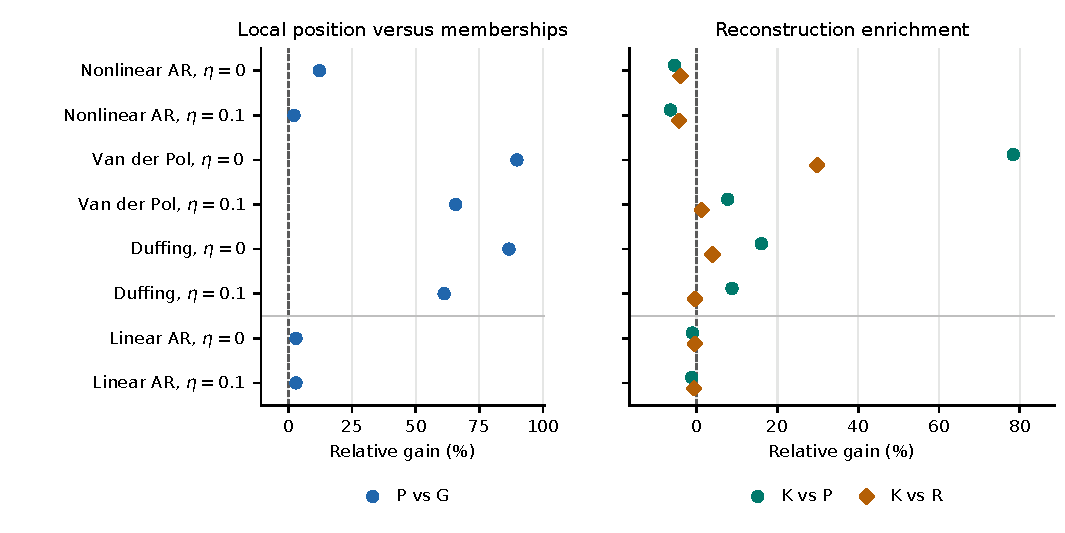
\includegraphics[width=\linewidth]{generated/soft_state_ablation/condition_gains.pdf}
\caption{Descriptive shared-cap gains computed from condition mean
losses. Positive values favor the first arm; dashed lines mark zero
gain. The last two rows are the linear controls, separated by a
horizontal rule. The horizontal scales differ between panels.
No confidence intervals or extra condition-specific superiority tests
are implied by these points.}
\label{supp:sa-condition-gains}
\end{figure}

\begin{table}[htbp]
\centering\small
\caption{Complete descriptive horizon-specific D SMSE means for the
nonlinear (NL) and linear (L) panels. Each horizon is normalized by
its corresponding A target variance before aggregation. The panel
means use equal law/noise weighting within each of
\SARepetitions\ repetitions. These are separately fitted direct
readouts, not successive steps of an autonomous rollout.}
\label{supp:sa-horizons}
% Generated by build_soft_state_assets.py; do not edit.
% Descriptive horizon-specific D SMSE; NL=nonlinear, L=linear. Per-horizon A target variances normalize loss.
\begin{tabular}{@{}llrrrrrr@{}}
\toprule
Cap rule & Arm & NL $h=1$ & NL $h=4$ & NL $h=12$ & L $h=1$ & L $h=4$ & L $h=12$ \\
\midrule
Shared & G & 0.0300446 & 0.0609004 & 0.205666 & 0.811376 & 0.999827 & 1.00592 \\
Shared & P & 0.0122551 & 0.0192541 & 0.059843 & 0.708544 & 1.00821 & 1.01601 \\
Shared & K & 0.0126386 & 0.0192272 & 0.0499322 & 0.718495 & 1.01811 & 1.02653 \\
Shared & R & 0.0120422 & 0.0186757 & 0.0511041 & 0.710428 & 1.01537 & 1.0218 \\
\addlinespace
Independent & G & 0.0300446 & 0.0609004 & 0.205666 & 0.811376 & 0.999827 & 1.00592 \\
Independent & P & 0.0122551 & 0.0192541 & 0.059843 & 0.708544 & 1.00821 & 1.01601 \\
Independent & K & 0.0123713 & 0.0190399 & 0.0488525 & 0.701798 & 1.01751 & 1.0255 \\
Independent & R & 0.0119662 & 0.018509 & 0.0497769 & 0.706971 & 1.01587 & 1.02483 \\
\bottomrule
\end{tabular}

\end{table}

\FloatBarrier
\subsection{Selected dimensions, numerical records, and computation}

The shared P-selected caps $1,2,4,8,12$ occurred in
$31,104,75,32,14$ of the \SATasks\ task suites, respectively.
Tables~\ref{supp:sa-selection} and \ref{supp:sa-selection-panels}
give both cap rules and the separate panel counts. G selected cap
one in every independent-cap task and its aggregate losses did not
change. P's shared and independent selections coincide by construction.
K and R often chose different caps under their own validation
objectives, so their independent-cap comparison no longer holds the
selected bank fixed.

At the shared bank, G used fourteen coordinates; P used $28$--$182$;
and K/R each used $196$--$350$, excluding the intercept. Centered
A feature ranks ranged from $9$--$11$ for G, $23$--$166$ for P,
$186$--$334$ for K, and $180$--$334$ for R. These widths do not
establish a compressed representation of the twelve-dimensional
history. Matching K/R widths does not match their function classes
or effective rank. Five of the $17{,}920$ local-model/cap records
used the native rank-zero wrapper: the same one-reference local
model in one task at each of the five caps. No positive-rank model
required a projected-range reduction. The zero-rank case was retained,
not omitted from evaluation.

Table~\ref{supp:sa-resources} reports measured computation for the
complete search, including rejected candidates and shared bank work.
The summed fit wall time was $931.88$ seconds and the summed D
prediction wall time was $671.84$ seconds. These are sums over worker
tasks, not elapsed time of the three-worker stage. The largest
recorded worker peak RSS was \SAPeakWorkerRSSMiB\ MiB, not an estimate
of simultaneous aggregate memory. Portable NPZ states occupied
\SAStateNPZMiB\ MiB in total; these retain all candidate states
and are not the size of a minimal deployed model. C diagnostic work
is included in the fit totals. Production analysis, independent
auditing, reporting, and archive compression are outside these costs.

The retained analysis records all $76{,}800$ cap/arm/penalty/horizon
B scores as valid. Full numerical solver events, native dimensions,
finite-value safeguards, C predictions, and both selected D views
remain available in the numerical record. The independent audit
passed \SAAuditChecks\ checks across all \SATasks\ tasks. It
independently refitted $25{,}600$ B penalty-path arrays and replayed
$2{,}048$ selected C and $2{,}048$ selected D forecast arrays.
Maximum absolute prediction differences were $1.20\times10^{-11}$
for B, $2.43\times10^{-12}$ for C, and $5.59\times10^{-12}$ for D,
within the frozen replay tolerances $2\times10^{-7}$ relative and
$2\times10^{-9}$ absolute. Source, seal, and stored prefix hashes
were checked exactly; independent numerical replay used the stated
tolerances. The audit also verified references, native ranks, gate
normalization, block transformations, selected penalties, and the
complete primary statistics. There were \SASolverRecoveries\ recorded
SVD-solver recoveries. Its receipt is bound by SHA256 to the released
analysis summary. This is computational verification of the retained
cohort, with the source-order and generator-scope limitations above.

\begin{table}[t]
\centering\small
\caption{B-selected cap frequencies across all \SATasks\ task suites
and selected feature-width/rank ranges. Cap columns count tasks;
the independent inferential sample is still \SARepetitions\
repetitions. Width excludes the intercept, and rank is the centered
A feature-matrix rank. Repeated shared rows reflect one P-selected
bank. Cap twenty is an alias of twelve, not an additional candidate.}
\label{supp:sa-selection}
% Generated by build_soft_state_assets.py; do not edit.
% B-selected cap counts across all 256 task conditions (not independent inferential units); width excludes intercept; centered feature rank on A.
\begin{tabular}{@{}llrrrrrcc@{}}
\toprule
Cap rule & Arm & 1 & 2 & 4 & 8 & 12 & Width range & Rank range \\
\midrule
Shared & G & 31 & 104 & 75 & 32 & 14 & 14 & 9--11 \\
Shared & P & 31 & 104 & 75 & 32 & 14 & 28--182 & 23--166 \\
Shared & K & 31 & 104 & 75 & 32 & 14 & 196--350 & 186--334 \\
Shared & R & 31 & 104 & 75 & 32 & 14 & 196--350 & 180--334 \\
\addlinespace
Independent & G & 256 & 0 & 0 & 0 & 0 & 14 & 9--11 \\
Independent & P & 31 & 104 & 75 & 32 & 14 & 28--182 & 23--166 \\
Independent & K & 67 & 57 & 73 & 42 & 17 & 196--350 & 181--334 \\
Independent & R & 59 & 75 & 89 & 16 & 17 & 196--350 & 177--334 \\
\bottomrule
\end{tabular}

\end{table}

\begin{table}[t]
\centering\small
\caption{Descriptive cap counts separated by population and selection
rule. The nonlinear rows contain $192$ law/noise/repetition task
conditions and the linear rows contain $64$; both populations have
\SARepetitions\ independent repetition units.}
\label{supp:sa-selection-panels}
% Generated by build_soft_state_assets.py; do not edit.
% Descriptive cap counts: 192 nonlinear and 64 linear task conditions, each arising from 32 repetitions.
\begin{tabular}{@{}lllrrrrr@{}}
\toprule
Population & Cap rule & Arm & 1 & 2 & 4 & 8 & 12 \\
\midrule
Nonlinear & Shared & G & 25 & 89 & 61 & 14 & 3 \\
Nonlinear & Shared & P & 25 & 89 & 61 & 14 & 3 \\
Nonlinear & Shared & K & 25 & 89 & 61 & 14 & 3 \\
Nonlinear & Shared & R & 25 & 89 & 61 & 14 & 3 \\
Nonlinear & Independent & G & 192 & 0 & 0 & 0 & 0 \\
Nonlinear & Independent & P & 25 & 89 & 61 & 14 & 3 \\
Nonlinear & Independent & K & 66 & 55 & 50 & 18 & 3 \\
Nonlinear & Independent & R & 56 & 64 & 66 & 4 & 2 \\
\addlinespace
Linear & Shared & G & 6 & 15 & 14 & 18 & 11 \\
Linear & Shared & P & 6 & 15 & 14 & 18 & 11 \\
Linear & Shared & K & 6 & 15 & 14 & 18 & 11 \\
Linear & Shared & R & 6 & 15 & 14 & 18 & 11 \\
Linear & Independent & G & 64 & 0 & 0 & 0 & 0 \\
Linear & Independent & P & 6 & 15 & 14 & 18 & 11 \\
Linear & Independent & K & 1 & 2 & 23 & 24 & 14 \\
Linear & Independent & R & 3 & 11 & 23 & 12 & 15 \\
\bottomrule
\end{tabular}

\end{table}

\begin{table}[t]
\centering\small
\caption{Whole-search resource measurements. All four arms, candidate
caps, and penalties share computations. Task sums of wall time are
not parallel elapsed times; peak worker RSS is not aggregate
concurrent memory. State sizes include all candidates and exclude
the separate retained prediction/data archives. These measurements
do not rank isolated arm costs or establish equal-compute comparisons.}
\label{supp:sa-resources}
% Generated by build_soft_state_assets.py; do not edit.
% Complete search/all four arms. Summed worker wall time is not parallel elapsed time; RSS is not concurrent aggregate memory; state sizes retain all candidates.
\begin{tabular}{@{}lrrr@{}}
\toprule
Measured quantity & Task sum & Task median & Task maximum \\
\midrule
Whole fit wall time (s) & 931.88 & 3.63 & 4.75 \\
Whole fit CPU time (s) & 929.02 & 3.62 & 4.65 \\
D prediction wall time (s) & 671.84 & 2.64 & 3.44 \\
D prediction CPU time (s) & 670.60 & 2.64 & 3.43 \\
Peak worker RSS (MiB) & --- & 155.88 & 156.99 \\
All-candidate NPZ states (MiB) & 177.93 & 0.69 & 0.70 \\
All-candidate JSON states (MiB) & 88.24 & 0.34 & 0.34 \\
\bottomrule
\end{tabular}

\end{table}
\FloatBarrier
